\section{Reunião 09 08 21 - Ronie e Pedro}

	\subsection{Mudanças no Gerenciar Unidades Solicitantes}
	
	\mssim Fica apenas Gerenciar Unidades.
	
	Ao cadastrar uma unidade, deve-se especificar se a Unidade é Interna ou Externa.

	Default é ser externa.
	
	Coloca um Boolean Interno? Não = Falso = 0 é o Padrão.
	
	Sim = True = 1 é porque é Interna.
	
	E aí deixa pré-cadastrada as 6 unidades internas: ASSEL, UDA, UCJ, UEF, URP, USE; 
		
	\begin{funcionalidade}{Cadastro de Unidades Externas}
		As unidades externas serão cadastradas ao longo do uso do sistema através de uma solicitação formal dessas unidades via SEI na qual deverá ser informado um (ou mais) usuários administradores.
	\end{funcionalidade}
	
	\textbf{Campos do Gerenciar Unidades}
	
	\begin{itemize}
		\item SIGLA : String;
		\item Nome da Unidade: String;		
		\item Interno: Booleano;
	\end{itemize}
	
	A Cardinalidade do Usuário e das Unidades será de muitos para muitos. Ou seja, um usuário pode ser cadastrado em várias unidades.	E uma unidade pode conter diversos usuários cadastrado nela.		

	\subsection{Mudanças na Tela de Login}
	
	\mssim Remover Combobox de escolha da Unidade.

	\begin{pergunta}{Para Gilberto}
		\mssim \textbf{Unidades Internas da ASSEL (ASSEL, UDA, UCJ, etc) tb fazem solicitações à ASSEL?} Independente da resposta, isto pode ser possível no futuro. Por enquanto não será, mas se precisar ser, será fácil fazer essa alteração.	

		
		\mssim \textbf{Existe a possibilidade de existir uma pessoa com trabalho em mais de uma unidade da ASSEL. Por exemplo? Trabalhar na ASSEL e na UDA ao mesmo tempo? Ou trabalhar na UDA e revisar na UCJ?} O sistema será modelado para permitir que isso seja feito, mas isso não vai ocorrer nesse início.		
	\end{pergunta}	

	
	\begin{imagine}{Tela de Login}
		A tela de login terá apenas o login e a senha.
		
		Ao fazer Login:

		\begin{enumerate}

		
		\item O sistema verifica se o usuário está cadastrado. Se não, não faz login, se sim segue com a verificação. Ao verificar, a pesquisa já trás em quais unidades o Usuário foi cadastrado.
		
		\item  Se existir um ou mais, adiciona essas unidades na lista.
		
		\item O sistema então verifica os resultados da lista:
		
		\begin{itemize}
			\item Tamanho da Lista = 0. Não entra pois não tem unidade associada. Mensagem de erro.
			
			\item Apenas 1 unidade. Loga na tela dessa unidade direto. Seja externo ou interno.
			
			\item Mais de uma unidades. Entra na tela de escolha da unidade que o usuário terá de escolher em qual unidade deseja logar-se. As possíveis unidades externas e internas aparecerão juntas na lista.
		\end{itemize}	

		\end{enumerate}
	\end{imagine} 

	
    \begin{figure}[htbp!]
		\centering
		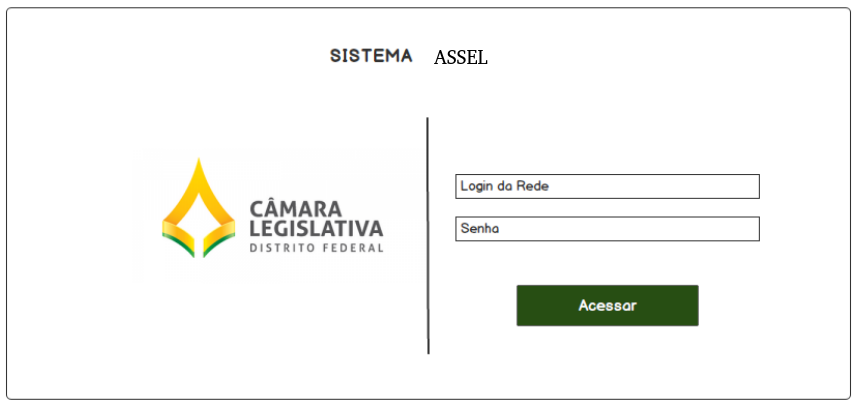
\includegraphics[width=0.8\textwidth]{fig/S1/fig-login.png}
		\caption{Tela de Login Principal}
	\label{fig:login}
	\end{figure}


	\subsection{Mudanças no Gerenciar Usuário}	
	
	Um Usuário pode estar vinculado com diversas Unidades.
	
	Então não existe mais o tipo "Externo".
	
	Pedro precisa fazer algumas mudanças lá.


	\subsection{Gerenciar Perfil}	
	
	 Parece OK
	 
	\subsection{Gerenciar Ordem de Serviço}		 
	
	\begin{enumerate}
		\item Listar - Cancelar e Abortar saem e agora é só Cancelar. O sistema verifica qual é o caso e quais são as operações.
		
		\item \textbf{Incluir e Visualizar}
		
		\begin{itemize}
			\item Quero uma tela só para incluir os Anexos um de cada vez.
			
			
			A estrutura de um Artefato é:
			\begin{itemize}			
				\item Anexo (Arquivo PDF, Imagem, Video, Etc...) - User Escolhe;
				\item Quem incluiu - Sistema registra;
				\item Data e Hora da Ultima Modificação - Sistema Registra;
				\item Nivel de Acesso (Publico ou Restrito) - User Escolhe;
				\item Justificativa Legal Se Restrito - User Escolhe;
				\item Tipo de Artefato (Inicial, Final, Pensar depois em mais casos) - Sistema Define;
				\item Descrição - User Escolhe;
			\end{itemize}		
			
			
			\item Os anexos deverão ser tratados já como Artefatos do Pacote de Artefatos vinculado a essa OS.
			
			
			\item A Especificação de Trabalho deve mostrar o \textbf{Textofato} do Tipo ``Especificação de Trabalho'' mais recente.
			
			
			A estrutura de um Textofato é:
			\begin{itemize}			
				\item Texto - User Escolhe;
				\item Quem incluiu - Sistema Registra;
				\item Data e Hora da Inclusão - Sistema Registra;
				\item Tipo de Textofato - Sistema Define;
			\end{itemize}		
			
			
		\end{itemize}
	\end{enumerate}
